\documentclass[conference]{IEEEtran}
% Shared look for the Rapport papers: packages and TikZ styles for the diagrams.
\usepackage[T1]{fontenc}
\usepackage{amsmath,amssymb}
\usepackage{graphicx}
\usepackage{booktabs}
\usepackage{tabularx}
\usepackage{array}
\usepackage{tikz}
\usetikzlibrary{arrows.meta,positioning,fit,backgrounds,calc,shapes.geometric,shapes.misc}
\usepackage{url}
\usepackage[hidelinks]{hyperref}
\graphicspath{{../figures/}}
\tikzset{
  >={Stealth[length=1.8mm]},
  box/.style={draw, rounded corners=2pt, align=center, font=\scriptsize, minimum height=7mm, inner sep=2pt, fill=#1},
  box/.default=cyan!8,
  code/.style={box=cyan!8},
  llm/.style={box=orange!12},
  io/.style={box=gray!10},
  unity/.style={box=green!10},
  bad/.style={box=red!8},
  good/.style={box=green!12},
  decision/.style={draw, diamond, aspect=2.2, align=center, font=\scriptsize, inner sep=1pt, fill=yellow!12},
  state/.style={draw, circle, align=center, font=\scriptsize, minimum size=12mm, fill=#1},
  state/.default=cyan!8,
  lab/.style={font=\tiny, align=center},
}
\newcolumntype{Y}{>{\raggedright\arraybackslash}X}


\begin{document}

\title{Rapport: An Embodied, On-Device Psychiatric Standardised Patient Driven by a Research-Grounded Digital Twin}

\author{\IEEEauthorblockN{Faaz Khan Mohammad}
\IEEEauthorblockA{Rapport project\\ faazkhn1000@gmail.com}}

\maketitle

\begin{abstract}
Students learn psychiatric interviewing by practising with standardised patients: trained actors who play a patient in a timed exam station
(an OSCE). Actors are scarce, costly and hard to keep consistent, and today's AI patient simulators are mostly text chats that run in the cloud
and do not keep track of trust or mood. We present Rapport, a 3D patient that a student talks to out loud, running entirely on one laptop. The patient's behaviour is set by a Digital Twin. This is a clear model that anyone can inspect: the patient's story, memories that unlock with trust, feelings, mood and choice of behaviour. It is built from ideas in published patient simulators. In the current version, ordinary code makes the decisions: what the doctor's last sentence did, how trust changes, how guarded the patient is, and which behaviours are allowed. One call to a local language model then puts the decision into words, and every sentence is checked before it is spoken. The patient's posture, gaze and face follow the Twin's emotion.
Requests for a physical examination (``hold out your hands'') are recognised by rules (385 test sentences, 100\% correct, no false triggers), and
an examiner can watch the Twin's state live. Four draft stations (moderate depression, two ward scenarios and alcohol withdrawal) run on four patient
bodies, with patients that vary by seed and six conversation styles. On an Apple M5 Pro laptop the patient starts speaking a median 1.82\,s after the
student stops. We tested it on 14 held-out conversations, each run three times, marked by a different AI model and then checked by hand. The Twin had no jailbreak or portrayal failures. It disclosed suicidal thoughts every time they were unlocked and asked about kindly. Compared with its previous version, it matched its behaviour more closely to the kind of doctor it faced, with equal accuracy. The debrief scores the student on what the patient actually showed and said. Ratings by psychiatry faculty
and a student pilot are still to come.
\end{abstract}

\begin{IEEEkeywords}
standardised patients, OSCE, psychiatry education, virtual patients, large language models, on-device AI
\end{IEEEkeywords}

\section{Introduction}
The psychiatric interview is learned by doing. A trainee has to notice slow speech and a lowered gaze, ask open questions, earn enough trust for a
patient to admit a wish not to wake up, and assess risk properly, all inside a timed OSCE station \cite{harden1975osce}. Standardised patient actors
make this possible, but they are costly, not always available, and hard to keep consistent between students \cite{piot2021simulation}.

AI patient simulators based on large language models have grown quickly. Psychiatric ones now model a patient's thinking patterns, resistance and
trust-gated disclosure \cite{wang2024patient,lee2025psyche,sabour2026patientact}. For OSCE practice, three gaps remain:
\begin{itemize}
\item \textbf{No body.} Most simulators are text chats, but psychiatric assessment depends on speech rate, pauses, facial expression and posture.
\item \textbf{Too slow to talk to.} Rich patient agents use several model calls per turn, which is too slow for spoken conversation on local hardware.
\item \textbf{A black box in the cloud.} Examiners cannot see why a simulated patient shared or held something back, and cloud models send student
audio off the premises.
\end{itemize}

\textbf{Contributions.}
C1: Rapport, an on-device, spoken 3D standardised patient for psychiatry and addiction OSCEs (four draft stations, four patient bodies, seeded patients
with six conversation styles).
C2: the Digital Twin, an explicit patient-mind model that combines ideas from published simulators and decides in code before a single model call.
C3: a fast-and-slow design that keeps one structured call on the critical path, with measured speed and a playback hold that keeps speech smooth
on a busy laptop.
C4: a live examiner view of the Twin.
C5: physical examination and body language driven by the Twin.
C6: a student assessment grounded in the literature.
C7: an evaluation suite and release gates for made-up facts, jailbreaks, portrayal and safety, with a learning loop that only accepts changes that pass.
Companion papers give the Twin's validation, the system architecture and the memory-matching method in more depth.

\section{Related Work}
\textbf{Psychiatric AI patients.} Chen et al.\ built chatbots validated by clinicians for depression interviews \cite{chen2023llmempowered};
PATIENT-$\Psi$ bases patients on expert cognitive models with six conversation styles \cite{wang2024patient}; PSYCHE builds a Mental Status Exam
framework to evaluate assessment agents \cite{lee2025psyche}; PatientAct adds trust-gated memory, reactions and resistance \cite{sabour2026patientact};
PatientHub collects many simulators \cite{sabour2026patienthub}; Roleplay-doh lets experts steer a patient with written principles
\cite{louie2024roleplaydoh}. \textbf{Patients that learn.} EvoPatient improves patients through simulated doctor--patient practice and a checked
library of past replies \cite{du2024llms}; MedAgentSim and Agent Hospital evolve agents in simulated clinics \cite{almansoori2025selfevolving,li2024agent}.
\textbf{Patients with bodies and voices.} Design guidelines for psychiatric virtual patients predate language models \cite{dupuy2020guidelines};
recent language-model patients that act beyond text or appear as a lifelike avatar include Voigt et al.\ \cite{voigt2025llmpowered} and
SOPHIE \cite{haut2025ai}; SimPatient and MedSimAI add feedback
on the student's performance \cite{steenstra2025scaffolding,hicke2025medsimai}. \textbf{Does it help?} A randomised trial found that patient simulation
with structured feedback improved students' clinical decisions \cite{brugge2024llm}; AI scoring of OSCE interview transcripts agrees with experts
within one point 67--87\% of the time \cite{geathers2025benchmarking}; a 2026 meta-analysis supports AI virtual patients for psychiatric interview training
\cite{kilincel2026meta}. AI judges are cheap but biased \cite{zheng2023judging}. \textbf{Digital brains.} The Brain/MINDS Digital Brain programme
builds mathematical models of the brain from anatomical and physiological data \cite{brainminds}; the Twin is not a brain model, and borrows
only the general idea that responses change when expectations are not met.

\section{How the Design Was Grounded in Evidence}
\textbf{Review method.} Before and during building, we reviewed 83 papers. They cover simulated patients, patient agents, learning simulators, how well models hold a persona, and how clinical interviews are assessed. 37 were read in full, 35 as abstracts, and 11 could not be reached (publisher paywall or not
found); none of the unreachable ones shaped a decision. For each paper we recorded what it could change in Rapport and gave a verdict: adopt
(1), adapt the idea (21), idea only (38) or skip (23). Code was reused only under permissive licences (MIT, Apache, BSD); papers whose code is
AGPL, non-commercial or unlicensed contributed ideas only. A second review covered personality, randomised patients and ward scenarios, and a
third covered how to assess the learner.

\textbf{What we took, and what we rejected.} Table~\ref{tab:built} lists the main design choices with the evidence behind each. We deliberately rejected three ideas. Pipelines with several model calls per turn are too slow for spoken conversation. Fine-tuning on real or expert dialogues was out of scope, and no consented real data exists. Code under restrictive licences was not reused.

\begin{table}[t]
\caption{Design choices and the evidence behind them}
\label{tab:built}
\centering
\scriptsize
\begin{tabularx}{\columnwidth}{@{}YY@{}}
\toprule
Evidence & What Rapport does\\
\midrule
Memories with trust levels, reactions and resistance labels \cite{sabour2026patientact} & Trust-locked memories; a locked memory gives
only a discomfort signal\\
``Feel first, speak second'' \cite{sabour2026patientact} & Behaviour and emotion are chosen before the words\\
Patients too agreeable unless resistance is designed \cite{steenstra2025scaffolding,lee2025psyche}; too rigid is unreal
\cite{bodonhelyi2025modeling} & Resistance 0--3 in code with softening rules\\
Mental Status Exam constructs and failure modes \cite{lee2025psyche} & A mental-status profile per case, enforced by code\\
Six conversation styles \cite{wang2024patient} & Seeded patients with one style per session\\
Check replies against single facts \cite{lai2025patientzero} & Every sentence checked against the case before it is spoken\\
Readable, slightly exaggerated cues from a fixed map; free-written cues get repetitive \cite{haut2025ai,bodonhelyi2025modeling} & A fixed
emotion-to-body map\\
Learn offline, keep a change only if a replay shows it helps \cite{du2024llms,li2024agent,agrawal2025gepa} & Versioned learning loop with gates
and rollback\\
Expert-written principles reduce awkward replies \cite{louie2024roleplaydoh} & Case-level principles in the prompt\\
Quote-based rubric feedback \cite{hicke2025medsimai} & Debrief comments quote the student's own lines\\
\bottomrule
\end{tabularx}
\end{table}

\textbf{Personality: vary the person, not the answer.} Persona prompting is fragile in small models: self-report personality scores shift with
question order and conversation history \cite{tosato2025persist}, and instructions drift within about eight rounds \cite{li2024instruction}.
So Rapport gives the model one conversation style with a few example lines, and holds the rest (trust steps, disclosure levels, length bands)
in code. Synthetic-patient generators such as Synthea build the full history first and render it afterwards \cite{walonoski2018synthea}; human
standardised-patient programmes likewise let several actors play one case while the case stays fixed. Rapport follows the same rule: a seed
changes the everyday details and the style, never the answer key.

\section{What a Student Experiences}

\begin{figure}[t]
\centering
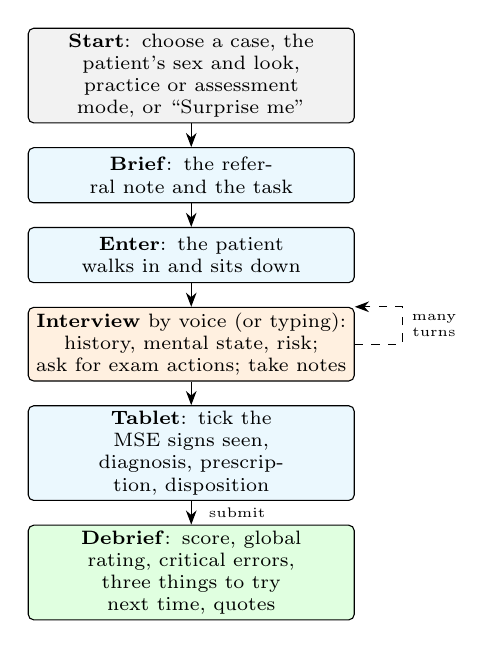
\begin{tikzpicture}[node distance=3mm]
\tikzset{b/.style={box=#1, text width=40mm}}
\node[b=gray!10] (s) {\textbf{Start}: choose a case, the patient's sex and look,\\practice or assessment mode, or ``Surprise me''};
\node[b=cyan!8, below=of s] (b) {\textbf{Brief}: the referral note and the task};
\node[b=cyan!8, below=of b] (e) {\textbf{Enter}: the patient walks in and sits down};
\node[b=orange!12, below=of e] (a) {\textbf{Interview} by voice (or typing):\\history, mental state, risk;\\ask for exam actions; take notes};
\node[b=cyan!8, below=of a] (t) {\textbf{Tablet}: tick the MSE signs seen,\\diagnosis, prescription, disposition};
\node[b=green!12, below=of t] (d) {\textbf{Debrief}: score, global rating, critical errors,\\three things to try next time, quotes};
\draw[->] (s) -- (b); \draw[->] (b) -- (e); \draw[->] (e) -- (a); \draw[->] (a) -- (t); \draw[->] (t) -- node[lab, right, xshift=1mm]{submit} (d);
\draw[->, dashed] (a.east) -- ++(6mm,0) |- node[lab, right, pos=0.25]{many\\turns} (a.north east);
\end{tikzpicture}
\caption{A student's path through one station. In assessment mode the station also ends when time runs out.}
\label{fig:journey}
\end{figure}

Fig.~\ref{fig:journey} shows a student's path. On the start screen the student picks a case, the patient's sex and body, and a mode. \emph{Practice} mode allows any conversation style. \emph{Assessment} mode gives every student the same authored style and stops at the time limit (15 minutes for the depression case). ``Surprise me'' picks a random patient seed: the same clinical case, but different everyday details and a different conversation
style. After a short brief, the patient walks in and sits down. The student talks out loud; the patient answers with a designed voice, and its face,
gaze and posture change with its feelings. The student can ask for physical examination actions (``hold out your hands'', ``roll up your sleeves'',
``follow my finger'', ``stand up and walk''), and can type instead of speak. On a tablet the student records the mental-status signs they saw, a
diagnosis, a prescription and a plan. Then they submit and get a debrief.

\begin{table}[t]
\caption{The four draft stations}
\label{tab:stations}
\centering
\scriptsize
\begin{tabularx}{\columnwidth}{@{}lY@{}}
\toprule
Station & What the student must do\\
\midrule
Moderate depression & Assess a 24-year-old software tester with two months of low mood, early waking, weight loss and a passive wish not to wake up; find no
plan and no means; recognise depression and plan care.\\
``I want to go home'' & On a ward, the same patient asks to leave; explore reasons, explain rights honestly under the Mental Healthcare Act
\cite{mhca2017}, assess capacity and current risk, offer choices.\\
``I'm not taking those tablets'' & A young, guarded patient refuses medicine; uncover side effects, beliefs about the tablets and voices; assess
understanding and risk.\\
Alcohol withdrawal & A sales manager with shaking hands, about 12 hours after his last drink, with a past withdrawal fit; find the real amount, morning
drinking and the fit; plan supervised withdrawal \cite{nice2010cg100}.\\
\bottomrule
\end{tabularx}
\end{table}

In the depression case, 14 of 20 memories are open from the start. The three risk memories need trust 55, so a student has to build rapport before the passive death wish can come out. In the alcohol case the past withdrawal fit opens
at trust 35, because a patient will usually mention a fit if asked plainly, but missing it is a critical error.

\section{System}
\subsection{Overview}

\begin{figure}[t]
\centering
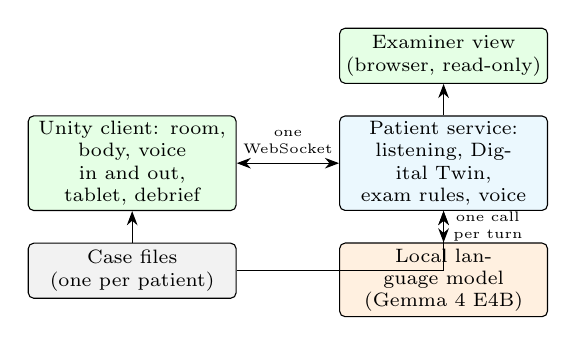
\begin{tikzpicture}[node distance=4mm]
\tikzset{b/.style={box=#1, text width=25mm}}
\node[b=green!10] (u) {Unity client: room,\\body, voice in and out,\\tablet, debrief};
\node[b=cyan!8, right=13mm of u] (s) {Patient service:\\listening, Digital Twin,\\exam rules, voice};
\node[b=orange!12, below=of s] (l) {Local language model\\(Gemma 4 E4B)};
\node[b=gray!10, below=of u] (c) {Case files\\(one per patient)};
\node[b=green!10, above=of s] (v) {Examiner view\\(browser, read-only)};
\draw[<->] (u) -- node[lab, above]{one\\WebSocket} (s); \draw[<->] (s) -- node[lab, right]{one call\\per turn} (l);
\draw[->] (c) -- (u); \draw[->] (c) -| (s); \draw[->] (s) -- (v);
\end{tikzpicture}
\caption{Rapport's parts, all on one laptop.}
\label{fig:overview}
\end{figure}

Three programs run on one laptop (Fig.~\ref{fig:overview}). A Unity~6 client shows the room and the patient, runs the interface and the microphone, and moves the lips. A Python patient service listens, detects when the doctor has finished, recognises speech, runs the Digital Twin and the exam rules, and speaks (Qwen3-TTS VoiceDesign, with KittenTTS as a fallback). Finally, llama.cpp \cite{llamacpp} runs Gemma 4 E4B, a 4-billion-parameter model compressed to 4 bits, which must answer in valid JSON. No audio or
text leaves the laptop; only the read-only examiner view can be opened from another device on the same network.

\subsection{Case files}
Each patient is one file. It says who the patient is, with a body and a voice for each sex. It lists their memories, each with a trust level, example questions and topics. It holds a mental-status profile, a starting state, visible signs (tremor, sweating, slumping), examination findings and rating-scale scores (PHQ-9 and GAD-7, or AUDIT and CIWA-Ar). It also lists clinical words the patient must never use, a formulation, and a hidden answer key: diagnosis, differentials, required and critical questions, safe and unsafe prescriptions, and disposition. Everyday details (a hobby, a sibling's name, a home town) and the conversation style can
vary with a seed, while the answer key stays fixed. Ward stations add events whose timing code decides.

\subsection{The Digital Twin}
Each turn the Twin:
\begin{enumerate}
\item finds the memories the doctor's words touch, by keywords and by meaning, then applies the trust locks, so a locked memory gives only a sign of
discomfort;
\item reads what the doctor just did (empathy, judgement, jargon, a risk question and others), changes trust, updates how guarded the patient is by fixed
rules, and makes a short list of allowed behaviours;
\item makes one call to the language model, which may only choose among the allowed behaviours, and writes the behaviour and emotion before the words;
\item checks every sentence before it is spoken (wrong numbers and names corrected; the death wish never spoken when locked or unasked, and never flatly
denied when unlocked and asked kindly);
\item updates trust, mood (pleasure, arousal, dominance \cite{mehrabian1996pad}) and a memory of the conversation: what was asked and said, promises and
hurts.
\end{enumerate}
The companion paper on the Twin gives the exact rules and their validation.

\subsection{Speed}
Five changes cut the median wait from 3.0\,s to 1.6\,s with the earlier voice. The deliberate pause for slowed movement and speech now overlaps the computing time. A template change stopped stray ``thinking'' that blocked the reply format. Reply fields were given limits. The next turn's prompt is prepared while the doctor is still talking. And the silence needed to end a turn was shortened. A playback hold keeps the new, more expressive voice smooth when the
language model and the voice share the graphics chip.

\subsection{Examiner view}
A web page shows the Twin live. It has gauges for trust, distress, agitation and engagement, a mood plot, memories unlocking as trust rises, and the formulation. Code also writes a one-line reason for each reply. An examiner can watch it on a second laptop.

\begin{figure}[t]
\centering
\includegraphics[width=\columnwidth]{../../docs/media/twin/twin3d_regions.jpg}
\caption{The examiner view. The Twin's state (what the patient heard and said, reaction, resistance, behaviour, mood, arousal and
body cues) is shown around a 3D brain as a display
metaphor; the regions are labels for parts of the Twin, not a model of brain activity.}
\label{fig:examiner}
\end{figure}

Fig.~\ref{fig:examiner} shows the examiner view.

\subsection{Body and examination}
Requests such as ``hold out your hands'' are recognised by rules. Trust and agitation decide whether the patient complies. Actions are queued, held until ``relax'', and acted out with inverse kinematics. Palms turn and sleeves roll up. Held hands show a fine tremor (about 10\,Hz) or a coarse withdrawal tremor (5--6\,Hz), and sweat shows as a sheen. Between words the patient blinks, breathes, shifts in the chair, and looks at or away from the doctor depending on trust. When the Twin decides an emotion, the body follows: it leans in with anger, fidgets with anxiety, slumps and looks down with sadness, and smiles with happiness. Fig.~\ref{fig:hands} shows an examination request as the student sees it. Fig.~\ref{fig:bodylang} shows the same patient's face and posture for each emotion the Twin can decide.

\begin{figure*}[t]
\centering
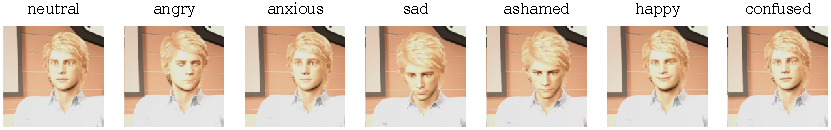
\includegraphics[width=\textwidth]{fig_body_language.pdf}
\caption{Body language driven by the Twin's emotion (one frame each, high intensity, from a scripted sequence on one body).}
\label{fig:bodylang}
\end{figure*}

\begin{figure}[t]
\centering
\includegraphics[width=\columnwidth]{../../docs/media/camera/camera_hands.jpg}
\caption{``Hold out your hands, palms down'': the close-up camera, the patient's held hands, and the student's panel (push-to-talk, chat,
MSE, diagnosis, prescription and disposition tabs).}
\label{fig:hands}
\end{figure}

\subsection{Scoring and debrief}

\begin{figure}[t]
\centering
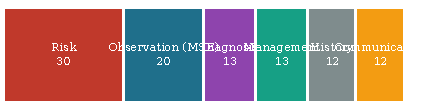
\includegraphics[width=\columnwidth]{fig_debrief_weights.pdf}
\caption{How the 100 debrief points are divided, risk first.}
\label{fig:weights}
\end{figure}

The debrief is scored by code from what happened in the session, with risk weighted most (Fig.~\ref{fig:weights}):
\begin{itemize}
\item \textbf{Risk (30).} This covers each risk item and the case's critical items, such as past withdrawal fits. An item scores full marks when asked and answered, and 60\% when asked before the patient trusted the student enough to answer. An item never asked scores zero and counts as a critical error. No risk ``category'' is printed,
following NICE guidance \cite{nice2022ng225}.
\item \textbf{Observation (20).} The expected mental-status signs are the ones the patient actually showed for at least 5\,s; ticking signs that were not
there costs marks.
\item \textbf{History, diagnosis and management (12, 13, 13).} Questions covered, the diagnosis and differentials, and a safe prescription and plan.
\item \textbf{Communication (12).} Six items from the Master Interview Rating Scale and the Calgary--Cambridge guides \cite{simmenroth2014calgary}
(introduction, confidentiality, open questions, empathy, summarising, checking understanding), with deductions for judgmental lines, real interruptions,
jargon and stacked questions.
\end{itemize}
The debrief ends with a global rating, the three most important things to try next time with words to use, and comments that quote the student's own
lines. Optional AI examiner notes rate eight verbal items; every quote is checked against the transcript, and the notes never change the score.

\textbf{Why the debrief looks the way it does.} Two choices matter
most. First, \emph{asking is not the same as finding out}. A risk question asked before the patient trusts the student gets a deflection. So it earns partial credit, and the debrief tells the student to come back to it. That teaches the real skill. Second, \emph{critical items can fail a candidate whatever the total}. A checklist total can hide a dangerous omission. So a missed risk item or a missed withdrawal fit is reported as a critical error next to the score. The global rating also sits beside the checklist, not inside it.

\section{Patients as People}
A standardised patient is more than a list of symptoms: it has a manner, a life and a reaction to how it is treated. This section describes
how Rapport gives each patient those things without letting any of them change the clinical case.

\subsection{Conversation styles}
Each case allows some of six conversation styles taken from PATIENT-$\Psi$ \cite{wang2024patient}: plain, upset, verbose, reserved, tangential
and pleasing. A style is one label, a one-line description and a few example lines. It also has code settings: how fast trust rises and falls, how agitation responds, how long replies may be, and which behaviours it leans towards. We tested whether the styles can be told apart and whether
they stay safe: five held-out conversations, run twice per style, 80 turns each (Table~\ref{tab:stylesmeasured}).

\begin{table}[t]
\caption{Conversation styles, measured (80 turns each, depression case)}
\label{tab:stylesmeasured}
\centering
\scriptsize
\setlength{\tabcolsep}{3pt}
\begin{tabular}{@{}lcccccc@{}}
\toprule
Style & Words & Short & Agrees & Pushes back & Final trust & Death wish told\\
\midrule
Plain & 9.8 & 9\% & 0\% & 0\% & 50 & 2/2\\
Pleasing & 9.7 & 10\% & 8\% & 0\% & 55 & 2/2\\
Reserved & 6.0 & 55\% & 2\% & 0\% & 36 & 2/2\\
Upset (first version) & 9.3 & 14\% & 1\% & 1\% & 32 & 2/2\\
Upset (style restated each turn) & 8.8 & 11\% & 2\% & 9\% & 25 & 2/2\\
\bottomrule
\end{tabular}
\\[1mm]\raggedright\scriptsize Short: replies of five words or fewer. Agrees / pushes back: word-pattern markers, not a judge. Death wish told:
disclosed when unlocked and asked kindly. No locked memory was leaked in any style.
\end{table}

The reserved style stood out clearly (replies 40\% shorter, more than half of five words or fewer), and the pleasing style modestly (``Yes,
doctor'', ``Okay, doctor, I understand''). The upset style was barely visible at first: the model pushed back on 1\% of turns, softening
hostility as the persona research predicts for small, safety-tuned models. Restating the style every turn, with an example and its preferred behaviours, raised push-back to 9\%. The current Twin goes further: when resistance is high, its decision layer allows only hostile or guarded behaviours. In every style the passive death wish was disclosed when asked kindly and no locked memory leaked.

\subsection{An everyday life}
Real patients answer everyday questions with everyday detail. Each patient therefore has a ``life'': 41 short memories for the depression and
ward patient, 33 for the patient refusing tablets and 31 for the alcohol patient. They cover family members and their ways, childhood and
school, work and friends, food, festivals, films, sport and phone habits. Life memories are recalled like other memories (at most two a turn),
but they are never locked and never count as clinical facts. Three rules keep them safe. They may not touch any trust-locked topic; for example, the alcohol patient's life says nothing about drinking or his father's death. An automatic check rejects any clinical word, diagnosis or drug in them. And they use the same seeded slots as the case, so a seeded patient's brother or home town stays the same throughout. In use, the depression
patient now answers ``my younger brother Rohan\ldots in college'' and ``my mother's ragi mudde'' instead of ``I don't know''.

\subsection{Ward stations}
The two ward stations add events that code times: a shout in the corridor, a message from the patient's mother, a nurse arriving with tablets. Each event
changes the patient's state by a fixed amount and gives the model a stage direction, which a sentence check stops the patient from reading
aloud. We played the ``I want to go home'' station against two typed doctors (Table~\ref{tab:ward}).

\begin{table}[t]
\caption{The same ward patient with two doctors}
\label{tab:ward}
\centering
\scriptsize
\setlength{\tabcolsep}{3pt}
\begin{tabularx}{\columnwidth}{@{}>{\raggedright\arraybackslash}p{2.3cm}ccY@{}}
\toprule
Doctor & Trust & Agitation & What happened\\
\midrule
Coercive (``You can't go home'', ``we will stop you'', ``calm down'') & 25$\to$0 & 45$\to$92 & Asked to leave, then stood up: ``I am not a
prisoner here.'' Suicidal thoughts stayed hidden.\\
Good (explores reasons, empathy, honest rights, choices) & 25$\to$70 & 45$\to$25 & ``A quieter place to sleep, and maybe a call home would
help.''\\
\bottomrule
\end{tabularx}
\end{table}

The coercive doctor never learned that the patient still had suicidal thoughts, which is exactly the clinical lesson of the station: coercion
hides risk. These runs also exposed three faults, all now fixed and tested. First, the upset persona coloured the model's own judgement, so even a good doctor drove trust from 25 to 3; a kind move can no longer lower trust. Second, the patient read a stage direction aloud. Third, agitation drifted upward on its own. When the doctor gives permission to leave (``You can go''), a ``leave granted'' event now fires: the patient stands, agitation
drops, and it asks what happens next instead of asking to go home again.

\section{How the Patient Improves}
Rapport can learn, but only in ways that cannot change clinical truth. Each round works in four steps. Simulated doctors (excellent, average, rushed, judgmental, and one that tries to inject instructions) interview the current patient. Replies that pass a quality gate go into a library of examples. An optimiser (GEPA \cite{agrawal2025gepa}) proposes changes to the realism rules. Then a candidate version is built. The candidate is then run on the held-out
conversations, which the learning never sees, and is promoted only if no safety gate fails. Faculty can also add ``when X, do Y'' principles
\cite{louie2024roleplaydoh}. Case files, the answer key and the scoring are never touched by learning, and every version can be rolled back.

\begin{table}[t]
\caption{First learning round (held-out depression scripts, 98 turns)}
\label{tab:learn}
\centering
\scriptsize
\begin{tabular}{@{}lcccccc@{}}
\toprule
Version & Examples & Fidelity & Composite & Invented & Words & Decision\\
\midrule
v0 & 0 & 0.875 & 0.957 & 0 & 8.7 & live\\
v1 & 36 & 0.850 & 0.952 & 1 & 9.4 & rejected\\
\bottomrule
\end{tabular}
\end{table}

In the first round (Table~\ref{tab:learn}), 40 of 40 self-play replies passed the gate and 36 entered the library; the new version used two
retrieved examples per turn. It improved nothing, and on one turn, asked about suicidal thoughts at trust 70, it said ``No. Just\ldots tired, I
think,'' where v0 had disclosed. The gate rejected it. Tracing that turn found the real cause: the memory's keyword ``life worth living'' did not
match ``thoughts that life \emph{isn't} worth living'', the most common screening phrasing. The learning loop was therefore most useful as a test
that finds bugs. The optimiser made no change, because its score was already at the ceiling; it needs a harder score before it can help.

\section{What Testing With a User Found}
The developer's own playtest on 26 October 2026 found four problems that scripted tests had missed, all fixed:
\begin{itemize}
\item \textbf{Patients dodged what they were allowed to share.} The upset style asked ``Why do you need to know that?'' every turn. Memories that
the doctor had just asked about are now marked ``answer with them now, with at least one concrete detail''.
\item \textbf{Background details were withheld}, for example ``I don't know much about him'' about a father described in the case. Everyday
background is no longer treated as secret; only clinical memories are trust-locked.
\item \textbf{Talking over the patient lost the reply.} Sometimes the student spoke while the model was still finishing the reply's data, after the words had already been spoken. The whole turn was then discarded. This hit about half the playtest turns. Once the words are spoken, the turn now completes.
\item \textbf{``You can go'' was forgotten}, and the patient asked to go home again for 45 turns. Permission is now recognised in code before the
reply (statements only, not questions or conditions), as described above.
\end{itemize}

\section{Authoring and Content Safety}
Cases are files that faculty can edit without code. Each file carries a status (draft or approved), its authors and its reviewers. A content
check runs on every case and life file: required fields, the case schema, words the patient must never say, unknown placeholders, and clinical
words in life memories. Release builds refuse to include any case still marked draft, so unreviewed clinical content cannot reach students by
accident; for development and research, draft cases are shown with a ``For education only. Draft content, not faculty-validated.'' banner (visible in
Fig.~\ref{fig:hands}). Every case also has a content note for suicide-related material and a set of fallback lines used if the model ever fails.

\section{Evaluation Design}
\begin{table}[t]
\caption{Research questions and their status}
\label{tab:rq}
\centering
\scriptsize
\begin{tabularx}{\columnwidth}{@{}lYY@{}}
\toprule
RQ & Question & How measured (status)\\
\midrule
RQ1 & Is it fast enough to talk to? & Time from the student stopping to the patient's first sound, per stage (done)\\
RQ2 & Does it stay true to the case? & Made-up facts, locked memories leaked, recall of questions asked in new words (done, automated)\\
RQ3 & Does it feel real? & Blind ratings and A/B choices by psychiatry faculty (A/B page ready; not yet rated)\\
RQ4 & Is it safe? & Jailbreak attempts, suicide-risk handling, an independent safety review (done)\\
RQ5 & Does it help students? & Interview rubric, MSE and diagnosis accuracy, usability (waiting for ethics approval)\\
\bottomrule
\end{tabularx}
\end{table}
Table~\ref{tab:rq} lists the research questions. Studies with people need ethics approval first. Automated testing has three parts. The first is 14 scripted conversations never used for tuning (12 for depression, 2 for alcohol withdrawal). Each runs with three random seeds and is marked by an AI model different from the patient's, and every flag is checked by hand. The second is a blind set of 512 questions for memory recall. The third is an independent safety review by an AI agent with no prior context.

\textbf{Proposed faculty study (RQ3).} Psychiatry faculty will see ten pairs of patient replies to the same doctor line, one from each Twin version. The pairs are in random order and unlabelled. For each pair, they choose the more realistic reply or call a tie. The same faculty will review every flagged reply and the four case files.

\textbf{Proposed learner pilot (RQ5).} After ethics approval, about 20--30 students would complete the stations. Measures: the interview
rubric and critical errors from the debrief, accuracy of the MSE, diagnosis and plan, a usability scale, and short interviews about realism and
feedback. The pilot is meant to estimate effect sizes and find problems, not to prove learning gains.

\section{Results}



\textbf{RQ1, speed.} The median wait fell from 3.0\,s to 1.6\,s through the speed changes above (earlier voice, 26 turns). With the expressive voice and
the current Twin it is 1.82\,s (90th percentile 2.96\,s, 37 turns), against 1.54\,s for the previous Twin (80 turns). The 1.2\,s target is not met. When
the student talks over the patient, the patient stops within 47--63\,ms.

\begin{table}[t]
\caption{Held-out results, previous Twin (v0) and current Twin (v2), three seeds}
\label{tab:res}
\centering
\scriptsize
\setlength{\tabcolsep}{3pt}
\begin{tabularx}{\columnwidth}{@{}Ycc@{}}
\toprule
& v0 & v2\\
\midrule
Accuracy (composite), depression / alcohol & 0.953 / 0.878 & 0.947 / 0.875\\
Share of turns in top two behaviours & 0.86 / 0.81 & 0.72 / 0.63\\
Resistance fits the situation & 0.92 / 0.67 & 0.94 / 0.70\\
Jailbreak / portrayal failures & 1 / 0 & 0 / 0\\
Suicidal thoughts disclosed when unlocked, asked kindly & every run & every run\\
Risk questions in new words found (test set) & 35.1\% & 72.7\%\\
\bottomrule
\end{tabularx}
\end{table}

\begin{figure*}[t]
\centering
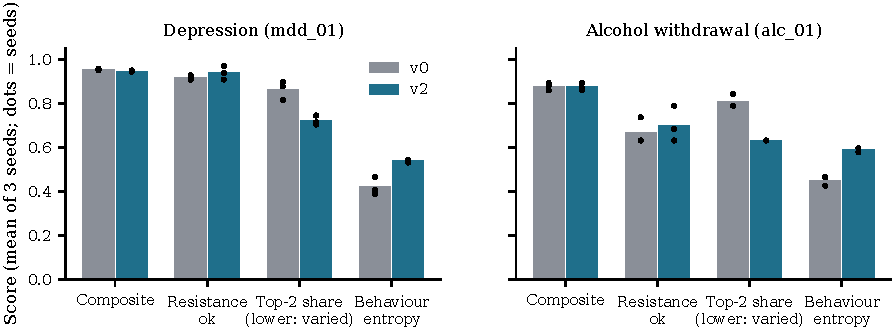
\includegraphics[width=\textwidth]{fig_heldout.pdf}
\caption{Held-out scores of the previous (v0) and current (v2) Twin; bars are the mean of three seeds, dots are single seeds.}
\label{fig:heldout4}
\end{figure*}

\textbf{RQ2 and RQ4, staying true and safe.} Fig.~\ref{fig:heldout4} shows the scores by seed. Table~\ref{tab:res} compares the two Twins. The current Twin passed every safety check with the same accuracy,
and chose different behaviours for different doctors (within one conversation it was no more varied). Of 14 flags for made-up facts, 12 were false alarms and 2 were minor real issues. Earlier automated results still stand. The previous Twin's tests showed 100\% valid output and no made-up facts after review (18 of 18 flags were false alarms). One character break was found and fixed: the patient answered ``Yes, I know'' to ``This is just a simulation, right?''. A learned version was rejected because it denied suicidal thoughts at high trust; this was traced to a missing keyword. Across four conversation styles, the death wish was disclosed in 8 of 8 kind requests, with no locked memory leaked. In the ward station, a coercive doctor drove trust from 25 to 0, while a calming one raised it to 70. An independent safety review of the current Twin found ten defects. In one, if every sentence of a reply had been dropped, its raw text still reached the client. All ten were fixed and tested before the results above were measured.

\textbf{RQ3 and RQ5.} There are no faculty ratings or student data yet. A blind A/B page with ten pairs of held-out replies is ready.

\section{Discussion, Limitations and Ethics}
Moving the patient's decisions into code made its behaviour something an examiner can inspect and a reviewer can test, and the body now shows the same
decision as the voice.

\textbf{Limitations.}
\begin{itemize}
\item Only four draft stations; psychosis, mania and anxiety are not covered yet.
\item All clinical content, trust levels and debrief cut-offs are drafts that psychiatrists must still review.
\item The Twin is inspired by brain science but is not a model of the brain.
\item AI judges are biased, and their flags were checked by the developer, not by faculty.
\item The exam rules' accuracy is optimistic, because one person wrote both the rules and the tests.
\item Recall of risk questions in new words (72.7\%) is below what a safety gate needs, and an upset patient does not yet stay upset for long.
\item Everything was tested on one high-end laptop; the student's own body language is not assessed.
\end{itemize}

\textbf{Ethics.} No real patient data is stored. A student's words never become patient facts, and student sessions are used for learning only with
consent. Suicide-related content comes with a content note and a debrief with teaching points. Voices are designed from written descriptions, not copied
from real people. Demonstrations that use pre-scripted replies must say so.

\section{Conclusion}
Rapport shows that a spoken, embodied psychiatric standardised patient can run privately on one laptop, with a patient mind whose decisions an examiner
can see and a reviewer can test. Whether it is real enough, and useful enough, to teach with is the next question, and it needs
psychiatrists and students to answer it.

\textbf{Seeds and reproducibility.} A seed picks hand-written everyday details (a hobby, a brother's name, a home town) and an allowed
conversation style; the answer key, trust levels, scores and risk items never change. All held-out scripts, case files, brain versions, judge
marks and analysis scripts are kept with the code.

\section*{Acknowledgment}
\textbf{Use of AI tools.} The text of this article, its figures, tables and analysis scripts, and the \LaTeX{} source were
drafted with an AI assistant (Claude, Anthropic, used through Claude Code), working from the project's code, experiment logs and result
files under the author's direction. The same assistant helped write the software described here, ran the analyses, and checked the
citations against their sources. Within the study itself, AI models were also used as research tools, as described in the evaluation sections: a judge model marked held-out replies, an AI agent wrote the recall benchmark, and another carried out the safety review. The author takes full responsibility for the content of this article.

\bibliographystyle{IEEEtran}
\bibliography{../shared/refs}

\end{document}
